\documentclass[12]{article}
\usepackage[left=1in,right=1in,top=1in,bottom=1in]{geometry}
\usepackage{amsfonts,amsmath,amssymb}
\usepackage{fancyhdr}
\usepackage{graphicx}
\usepackage{float}
\usepackage{transparent}
\usepackage{eso-pic}
\usepackage[tiny]{titlesec}
\usepackage{blindtext}
\usepackage{sectsty}
\usepackage{setspace}
\usepackage{titlesec}
\doublespacing
\usepackage{indentfirst}
\usepackage{makecell}
\sectionfont{\centering \normalsize \normalfont}
\usepackage{tocloft}
\renewcommand{\cftsecfont}{\normalsize \normalfont}
\renewcommand{\cftsecleader}{\normalsize \normalfont \cftdotfill{\cftdotsep}}
\renewcommand{\contentsname}{\hfill \normalsize \normalfont TABLE OF CONTENTS}
\renewcommand{\cftaftertoctitle}{\hfill}


\fancypagestyle{mypagestyle}{%
\fancyhf{} 
\renewcommand{\headrulewidth}{0pt}
\lhead{ \tiny \MakeUppercase{{\tiny   Exam Scheduling }}}
\rhead{}
\setlength{\footskip}{10pt}

\cfoot{\thepage}
}



\pagestyle{fancy}
\fancyhf{} 
\renewcommand{\headrulewidth}{0pt}
\lhead{ \MakeUppercase{{\tiny  Exam Scheduling}}}
\rhead{\scriptsize{\thepage}}

\renewcommand{\thesection}{\Roman{section}. } 
\renewcommand{\thesubsection}{\Alph{subsection}.}


\sectionfont{\centering\normalsize\normalfont\MakeUppercase}

\setlength{\headheight}{.5in}
\setlength{\headsep}{.5in}



\begin{document}
\begin{titlepage}

\pagenumbering{roman}

\setlength{\parindent}{0pt}
    \vspace*{-3.8\baselineskip}
    \MakeUppercase{{\tiny  Exam Scheduling}} \hfill 
    \begin{center}
    
    \vfill
     Solving Exam Scheduling Problem  Using Graph Coloring
\\
    \vfill
    
    A  Final Report\\
    \vfill
    
    Presented to  \\
    Professor Katerina Potika\\
    \vfill
    
    Department of Computer Science\\
    San Jos\'e State University\\
    \vfill
    
    In Partial Fulfillment\\
    Of the Requirements for the Class\\
    CS 255\\
    \vfill
    
    By\\ 
    Fei Pan,\\
    Joshua Benz\\
    30 April, 2019\\
\end{center}
\end{titlepage}

\tableofcontents
\thispagestyle{mypagestyle}
\clearpage
\pagenumbering{arabic}
\setcounter{page}{1}
\setlength{\parindent}{4em}
\renewcommand{\baselinestretch}{1.5}

\section{Introduction}
Graphs are useful data structures for modeling relationships between different types of data. The applications of graphs include modelling social media interactions , modelling maps for path optimizations, recommendation engines and more. Once a graph is constructed, there are a variety of algorithms that can be used to obtain information from them. In this project, we examine a special case known as graph coloring.

The graph coloring problem is to assign colors to every vertex in theo graph such that no adjacent vertices have the same color assignment. The goal of this problem is to minimize the number of colors needed to color the graph. Graph coloring is NP-Complete which means there is no polynomial time algorithm for finding the optimal solution. Therefore, we explore approximations. 

This project examines a Greedy approach, Welsh-Powell and a Genetic algorithm approach to obtaining a valid graph coloring for undirected graphs. All of these algorithms are approximations and do not guarantee optimal solutions. In the case of the genetic algorithm, it does not guarantee a solution at all. We will apply these algorithms to graphs that model university final exam scheduling.
\section{DEFINITION OF THE PROBLEM}
A graph is said to be colored if a color has been assigned to each vertex in such a way that adjacent vertices have different colors. And this process of assigning colors to the vertices of a graph is called graph coloring.

Suppose we want to schedule some exams for SJSU students. The problem can be converted into a graph coloring problem. Given a graph G(V, E), in which the vertices V represent courses and two vertices are connected as an edge E if the corresponding courses have a student in common. Two connected vertices should be colored differently. As in exam scheduling, no student will be scheduled to take two course exams simultaneously. The objective of this problem is to find a complete solution that every course is assigned to a time slot and a room, and to minimize the total number of time periods, which is represented as the chromatic number of a graph.

The objective of this problem is to find a complete solution that every course is assigned to a time slot and a room, and to minimize the total number of time periods / chromatic number of a graph.
\section{ALGORITHM DESCRIPTIONS}
\subsection*{Greedy}
\begin{enumerate}
	\item Select the first vertex and make it the first color
	\item For each vertex in the graph
	\begin{enumerate}
		\item Visit each neighbor and take note of the colors assigned to the neighbors
		\item Pick the first color that isn't assigned to a neighbor
	\end{enumerate}
\end{enumerate}

\subsection{Welsh-Powell}

\begin{enumerate}
\item Find the degree of each vertex
\item List the vertices in order of descending degrees.
\item Color the first vertex with color 1.
\item Move down the list and color all the vertices not connected to the colored vertex, with the same color.
\item Repeat step (1) on all uncolored vertices with a new color, in descending order of degrees until all the vertices are coloured.
\end{enumerate}

\subsection{Genetic Algorithm}
\begin{enumerate}
\item Create an initial population of genomes (randomly or not)
\item While Fitness is not 0 and we have not reached 20,000 iterations
\begin{enumerate}
	\item For each genome, do the following
	\begin{enumerate}
		\item Update its fitness score based on the number of bad edges
		\item If we have an optimal fitness score, stop the program
	\end{enumerate}
	\item Select two parents and do the following
	\begin{enumerate}
		\item Crossover the parents to make a new child
	\end{enumerate}
	\item Mutate the child
	\item Place the child in the population
	\item Place the fitter of the two parents into the population (this wasn’t specified, it’s just how I decided to do it)
\item If we reach 20,000 iteration, stop and perform wisdomOfTheArtificialCrowds
\end{enumerate}
\end{enumerate}

In this algorithm, a genome holds a chromosome and an associated fitness score. The chromosome is an array based representation of the coloring of the graph. The position in the array represents the vertex in the graph while the value at the position is the assigned color for that vertex. “Bad edges” are defined as edges between vertices of the same color. Parent selection is done by either selecting the top two performing genomes in the population or by randomly selecting two genomes from the population. Mutation is done by looking at a chromosome and looking and taking each position as a vertex. We get the neighbors of the vertex and keep track of what colors are used. At the end, the vertex gets assigned a random color out of the difference of AllColors - usedColors. In other words, pick a random color that isn’t used by any of the neighbors. WisdomOfTheArtificialCrowds is performed by taking the top performing chromosome and looking at its bad edges. Then you take the top 50$\%$ of performers and take a majority vote on what color they use that works. Then we assign that color for the vertex in the top performer. The size of the population, mutation rate and number of iterations were experimentally chosen.	


\section{IMPLEMENTATION DETAILS}
The above algorithms were implemented in python with use of the pandas library.
\begin{figure}[H]
\centering
        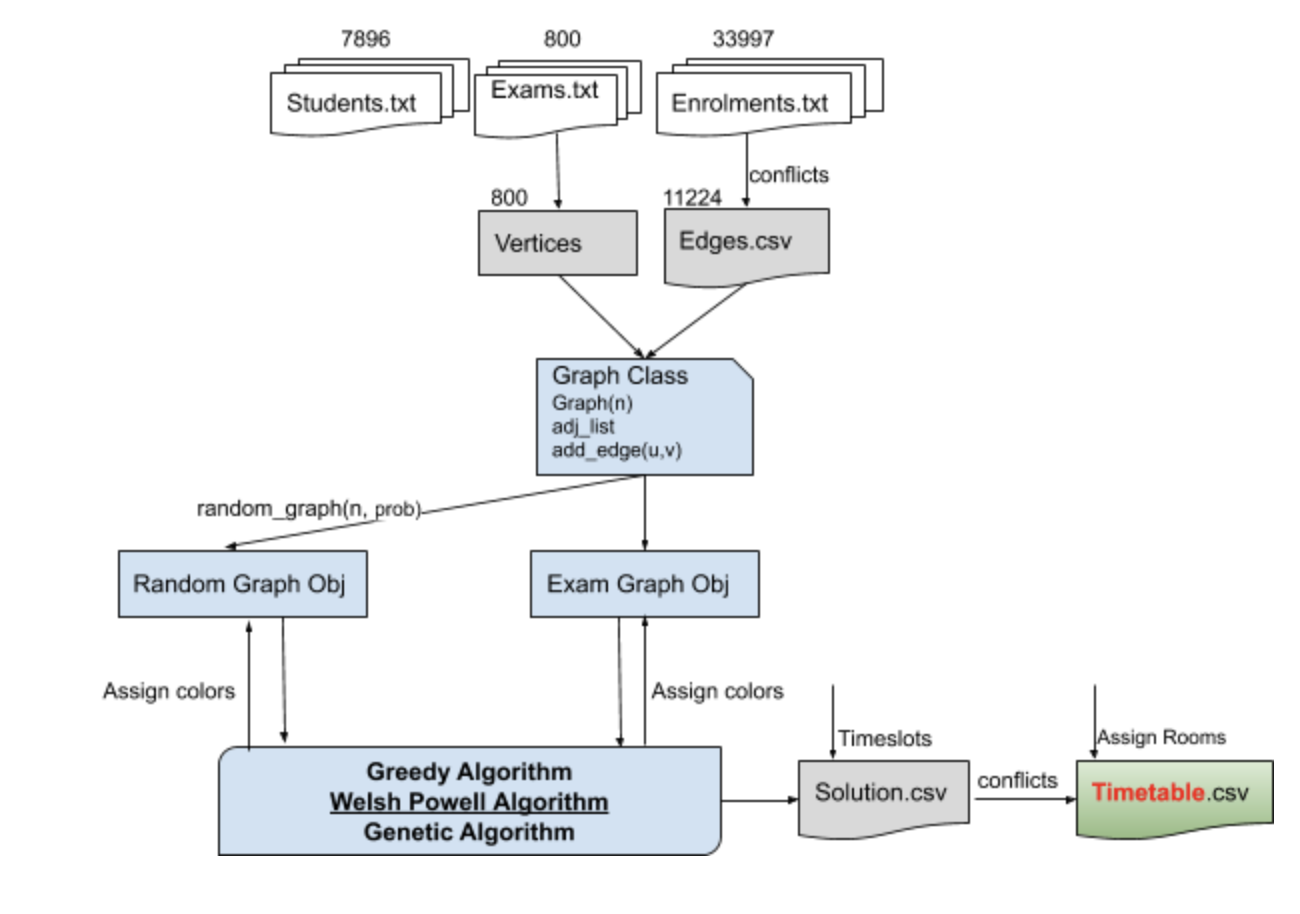
\includegraphics[scale=.35]{imp.png}
    \caption{Execution Flow}
\end{figure}
\section{RELATED WORK}
Graph coloring is an NP-Complete problem, so there has been a lot of work done to find better algorithms and special cases. In this paper we implemented the standard Greedy Algorithm, Welsh-Powell and Genetic algorithm. In this project we specifically implement....NUMBER
\section{DATA SETS USED}
\begin{enumerate}
\item This data is from the University of Nottingham, semester 1, 1994-95. There are 800 exams provided by 46 departments, and 7896 students. There are 33997 enrollments, so each student is sitting an average of 4.3 exams, and each exam is sat by an average of 42.5 students.

\item Graphs randomly generated by following the Erdős–Rényi model. This algorithm works by selecting the number of vertices and a probability of them being connected. Then I generated a random number and if it was less than or equal to the probability, then I added an edge between the vertices.
\end{enumerate}
\section{ANALYSIS AND COMPARISON}
\begin{table}[H]
\centering
\begin{tabular}{|l|l|l|l|}
\hline
  & \bf{Greedy}  & \bf{Welsh-Powell} &  \bf{Genetic}  \\ \hline
\makecell{\bf{Random Graph} \\ ($|V|$ = 800, $|E|$ = 12716)}\\  & \makecell{15}  & 13 &  -  \\ \hline
 \makecell{\bf{Exam Graph} \\ ($|V|$ = 800, $|E|$ = 11224)}\\ & 26  & 19 &  39  \\ \hline
\end{tabular}
\end{table}
\section{EXPERIMENTAL RESULTS}

\section{FURTHER DISCUSSION}
\subsection{Genetic Algorithm}
The genetic algorithm presented in the paper has some interesting properties. The optimal fitness score is defined to be 0, since that would mean there are no conflicting edges.  The authors present two different parent selection and mutation functions in an attempt to converge as quickly as possible. Despite trying to implement those functions, I was unable to reproduce the same benchmarks that were presented in the paper. However, I did try various ideas and with some fine tuning, I managed to get fairly decent performance. One problem that I currently have with it is the execution speed. Python isn't particularly fast, but I also am not familiar enough with the language to be able to optimize it enough. After profiling the code, I found that the bottleneck is from constantly getting the colors of adjacent edges. This also explains why the algorithm struggles with densely connected graphs.

There are some details left out of the paper as well. For example, they talk about parent selection, crossover, mutation and then adding the child to the population. However, they only add one child to the population while also mentioning that the population size should be constant. Therefore, I either need to repeat the process with another child so that I can replace both parents, or leave a parent in the population. I experimented with both. Creating two children made the fitness scores more erratic. This could potentially be beneficial since there is more exploration, but it seemed to converge onto a pattern. I think this would be a more feasible option if there was more randomness in play. The other option I explored was to take the fittest of the parents and put that parent back into the population. This had the effect of a slow, but steady decrease in the fitness score.

Bad edges are defined as edges between vertices of the same color. The fitness function is calculated by counting the number of bad edges. However, given enough colors and a large enough graph, this is pointless. For example, if I gave the genetic algorithm enough colors for each vertex, then the algorithm would converge in seconds, usually around 12 to 20 generations. However, the color assignment seems like it might be slightly better than trying to randomly assign colors. The result of this would usually be around 500 out of 800 colors. So perhaps an adjustment that can be made is to have a penalty for chromosomes that use a lot of colors. That way the fitness score improves when there are better assignments or there are less colors used or, ideally, both.

Another thing to take into consideration is the initial population. I tried assigning colors at random while also using all of the colors, assigning at random using a subset of colors and assigning all the vertices the same color. The initial assignment with all vertices the same color converged quickly at first, but then peaks. Assigning colors at random with a color for each vertex converges in about 10-20 generations but also uses about 500 colors. Finally, assigning the vertices at random, but only using a subset of the colors behaves similar to assigning them to one color.

I also  tried limiting the number of colors that were available to the algorithm. For example, giving the algorithm a set of 50 colors to work with in the exam graph of 800 vertices allows the algorithm to converge to a solution in about 20 generations. Giving it 35 colors makes it converge at around 50 to 200 generations.

Some other variables that I changed were the population size, mutation rate and crossover rate. Changing the population size didn't really help. Having a high mutation rate was good, but I found that 0.8 tends to work best with a crossover rate of 1.0. If the mutation rate was too high, it would often get to a good fitness score, but then get stuck.

Finally, I found that a mutation rate of 0.8 with a crossover rate of 1.0, population size of 50 and between 37-40 colors converges in a reasonable amount of time. However, the genetic algorithm performs poorly on random graphs since I can't really fine tune the parameters. So one of the downfalls of the genetic algorithm is that it sometimes requires fine tuning the parameters for specific examples.
\section{CONCLUSION}
\newpage
\section*{References}
\addcontentsline{toc}{section}{References}%
\renewcommand{\section}[2]{}%
\begin{thebibliography}{1}
\singlespacing


\bibitem{Goebel} R. Goebel, A. Chander, K. Holzinger, F. Lecue, Z. Akata, et al.. Explainable AI: the new 42?. 2nd Int. Cross-Domain Conf. for Mach. Learning and Knowl. Extraction (CD-MAKE), Aug 2018, Hamburg, Germany. pp 295-303, ff10.1007/978-3-319-99740-7$\_$21ff. ffhal-01934928f \\


  \bibitem{Hoffman} R. R. Hoffman, G. Klein, and S. T. Mueller, "Explaining explanation for “explainable AI”" in  \textit{Sage Journals}, vol.62 no. 1, pp. 197-201, Sept. 2018. [Online]. doi:10.1177/1541931218621047\\
  
    \bibitem{Kass} R. Kass, and T. Finin, "The need for user models in generatnig exper system explanations" 1988. [Online]. https://repository.upenn.edu/cis/\\

    \bibitem{Buchanan} B. G. Buchanan, and E. H. Shortliffe, "Rule-based expert systems:
The MYCIN experiments of the Stanford heuristic programming project" pp. 754 1984. [Online]. http://www.shortliffe.net/Buchanan-Shortliffe-1984/MYCIN\\


    \bibitem{Swartout} W. Swartout, C. Paris, and J. Moore, "Explanations in knowledge systems: design for explainable expert systems".  \textit{IEEE Expert} pp. 58–64 1991. [Online]. http://people.dbmi.columbia.edu/\\

    \bibitem{Bratko} I. Bratko, "Machine learning: between accuracy and interpretability". in \textit{Int. Centre for Mech. Sci.} vol 382 pp. 163-167 1997. [Online]. https://link.springer.com/chapter/10.1007/978-3-7091-2668-4$\_$10\\



\bibitem{Lou} Y. Lou, R. Caruana, and J.Gehrke. "Intelligible models for classification and regression". in  \textit{Proc. 18th ACM SIGKDD Int. Conf.  Knowl. Discovery and Data Mining}, 2012, pages 150–158. ACM.

  \bibitem{Ribeiro} M. T. Ribeiro, S. Singh, C. Guestrin, ""Why should I trust you?": Explaining the predictions of any classifier" in \textit{IEEE Access}, vol.6,  pp. 52138 - 52160, Sept. 2018. [Online]. doi: 10.1109/ACCESS.2018.2870052\\
  
    \bibitem{Montavon} G. Montavon, S. Bach, A. Binder, W. Samek, K. Muller, "Explaining non-linear classification decisions with deep taylor decomposition" in \textit{Pattern
Recognition},  pp. 211–222, 2017. [Online]. https://arxiv.org/abs/1704.04133\\

    \bibitem{Kumar} D. Kumar, A. Wong, G. W.  Taylor, "Explaining the unexplained: A class-enhanced attentive response (CLEAR) approach to understanding deep neural networks"  [Online]. https://arxiv.org/abs/1602.04938\\
    
        \bibitem{Lipton} Z. C. Lipton, "The mythos of model interpretability" in \textit{ICML Workshop on Human Interpretability in Mach. Learning (WHI 2016)}, 2016. [Online]. https://arxiv.org/abs/1606.03490\\

    \bibitem{Preece} A. Preece, "Asking 'why' in AI: explainability of intelligent systems - perspectives and challenges". [Online]. https://dais-ita.org/sites/default/files/2326$\_$paper.pdf\\

  \bibitem{Peeked} A. Adadi, M. Berrada, "Peeking inside the black-box: a survey on explainable artificial intelligence" in \textit{Proc. of the 22nd ACM SIGKDD Int. Conf. on Knowl. Discovery and Data Mining (KDD’16),}, pages 1135–
1144. ACM. 2016. [Online].https://dais-ita.org/sites/default/files/2326$\_$paper.pdf\\
  
    \bibitem{Chittajallu} D. R. Chittajallu, B. Dong, P. Tunison, R. Collins, k. Wells, et al., "XAI-CBIR: explainable AI system for content based retrieval of video frames from minimally invasive surgery videos" in \textit{2019 IEEE 16th Int. Symposium on Biomed. Imaging (ISBI 2019)}, April. 2019. [Online]. doi: 10.1109/ISBI.2019.8759428\\
  
  
    \bibitem{Kulikowski} C. A. Kulikowski, "Artificial intelligence methods and systems
for medical consultation " in \textit{IEEE Trans. Pattern Anal.  Mach. Intell.}, vol. PAMI-2, no. 5 pp. 464 - 476, Sept. 1980. [Online]. https://ieeexplore.ieee.org/document/6592368\\
  
      \bibitem{Long} J. M. Long, j. R. Slagle, M. Wick, E. Irani, j. Matts, et al. "Use of expert systems in medical research data analysis: The POSCH AI project ", vol.1, pp. 796. [Online]. doi: 10.1109/AFIPS.1987.120\\
  
        \bibitem{Ding} L. Ding "Human knowledge in constructing AI systems - neural logic
networks approach towards an explainable AI ", \textit{Int. Conf. Knowl. Based and Intell. Inf. and Eng. Syst.}, Sept. 2018. [Online]. https://app.dimensions.ai/details/publication/pub.1106387404?and$\_$facet$\_$journal=jour.1320495\\
  
        \bibitem{gunning}D. Gunning "Explainable artificial intelligence",  in \textit{DARPA/120}, Nov. 2017, [Online]. https://www.darpa.mil/attachments/XAIProgramUpdate.pdf\\
  
  
          \bibitem{Tjoa} E. Tjoa and C. Guan "A survey on explainable artificial intelligence (XAI): towards medical XAI", July. 2019, [Online]. https://arxiv.org/abs/1907.07374\\
  
  
            \bibitem{Doshi-Velez} F. Doshi-Velez and B. Kim "Towards a rigorous science of interpretable machine learning", Fep. 2017, [Online]. https://arxiv.org/abs/1702.08608\\
  
              \bibitem{Xie} Y. Xie, X. Chen, and G.Gao "Outlining the design space of explainable intelligent systems for medical diagnosis", March. 2019, [Online]. https://arxiv.org/pdf/1902.06019.pdf\\
  
  

  \end{thebibliography}
\end{document}